%%%%%%%%%%%%%%%%%%%%%%%%%%%%%%%%%%%%%%%%%%%%%%%%%%%%%%%%%%%%%%%%%%%%%%%%%%%%%%%%
% AMS Beamer series / Bologna FC / Template
% Andrea Omicini
% Alma Mater Studiorum - Università di Bologna
% mailto:andrea.omicini@unibo.it
%%%%%%%%%%%%%%%%%%%%%%%%%%%%%%%%%%%%%%%%%%%%%%%%%%%%%%%%%%%%%%%%%%%%%%%%%%%%%%%%
%\documentclass[handout]{beamer}\mode<handout>{\usetheme{default}}
%
\documentclass[presentation, 10pt]{beamer}\mode<presentation>{\usetheme{AMSBolognaFC}}
%\documentclass[handout]{beamer}\mode<handout>{\usetheme{AMSBolognaFC}}
%%%%%%%%%%%%%%%%%%%%%%%%%%%%%%%%%%%%%%%%%%%%%%%%%%%%%%%%%%%%%%%%%%%%%%%%%%%%%%%%

%\usepackage{lmodern}
\usefonttheme{professionalfonts}
\usepackage{arev}
\usepackage{multicol}
\usepackage{wasysym}
\usepackage{amsmath,blkarray}
\usepackage{centernot}
\usepackage{fontawesome}
\usepackage{fancyvrb}
\usepackage[ddmmyyyy]{datetime}
\renewcommand{\dateseparator}{}
%\renewcommand{\thefootnote}{\fnsymbol{footnote}}
\newcommand{\version}{1}
\usepackage{biblatex}
	\makeatletter

\addbibresource{biblio.bib}
%%%%%%%%%%%%%%%%%%%%%%%%%%%%%%%%%%%%%%%%%%%%%%%%%%%%%%%%%%%%%%%%%%%%%%%%%%%%%%%%
\title[Leveraging LLMs in Software Engineering]
{Leveraging Large Language Models in Software Engineering}
%
\subtitle[Research, Prospectives, Concerns]
{Research, Perspectives, Concerns}
%
\author[\sspeaker{Aguzzi}]
{\speaker{Gianluca Aguzzi} \href{mailto:gianluca.aguzzi@unibo.it}{gianluca.aguzzi@unibo.it}}
%
\institute[DISI, Univ.\ Bologna]
{Dipartimento di Informatica -- Scienza e Ingegneria (DISI)\\\textsc{Alma Mater Studiorum} -- Universit{\`a} di Bologna}
%
\renewcommand{\dateseparator}{/}
\date[\today]{\today}
%
%%%%%%%%%%%%%%%%%%%%%%%%%%%%%%%%%%%%%%%%%%%%%%%%%%%%%%%%%%%%%%%%%%%%%%%%%%%%%%%%
\begin{document}

\nocite{*}
%%%%%%%%%%%%%%%%%%%%%%%%%%%%%%%%%%%%%%%%%%%%%%%%%%%%%%%%%%%%%%%%%%%%%%%%%%%%%%%%

%/////////
\frame{\titlepage}
%/////////
%% print toc
\begin{frame}{Outline}
	\tableofcontents
\end{frame}
%===============================================================================

\section{Introduction to LLMs}
\begin{frame}{Today Lesson in a Nutshell}
	\centering
	
\includegraphics[width=0.5\textwidth]{img/meme.jpg}
\end{frame}
\begin{frame}[plain]
\centering
\huge{
	\textbf{Natural Language Processing} (NLP)
}
\\[1em]
\large{
	{A subfield of artificial intelligence that focuses \emph{understanding}, \emph{interpreting}, and \emph{generating} human language.}
}

\vspace{1em}
\small{
	\textbf{Resources}
	\begin{itemize}
		\item \url{https://github.com/keon/awesome-nlp?tab=readme-ov-file}
		\item \url{https://github.com/brianspiering/awesome-dl4nlp}
		\item \url{https://nlpprogress.com/}
		\item \url{https://www.unibo.it/it/studiare/dottorati-master-specializzazioni-e-altra-formazione/insegnamenti/insegnamento/2023/412644}
	\end{itemize}	
	
}
\end{frame}

\begin{frame}{Natural Language Processing}
	\begin{alertblock}{Goal}
		Identify the structure and meaning of \emph{words}, \emph{phases}, and \emph{sentences} in order to enable computers to understand and generate human language.
	\end{alertblock}
	\begin{exampleblock}{Why?}
		Improve \emph{human-computer} interaction, closing the gap between \emph{human communication} and \emph{computer understanding}.
	\end{exampleblock}
	\begin{alertblock}{Applications \textbf{(all around us)}}
		\begin{multicols}{2}
			\begin{itemize}
				\item \emph{Chatbots}
				\item \emph{Machine Translation}
				\item \emph{Speech Recognition}
				\item \emph{Sentiment Analysis}
				\item \emph{Question Answering}
				\item \emph{Code Generation}
			\end{itemize}
		\end{multicols}
	\end{alertblock}
\end{frame}
\begin{frame}{Natural Language Processing}
    \begin{alertblock}{Challenges}
        \begin{itemize}
            \item \textbf{Ambiguity:} Multiple meanings for words/phrases.
            \item \textbf{Context:} Meaning shifts with context (linguistic, cultural).
            \item \textbf{Syntax:} Sentence structure affects meaning.
            \item \textbf{Sarcasm/Idioms:} Non-literal language interpretation.
        \end{itemize}
    \end{alertblock}
    \begin{exampleblock}{Approaches}
        \begin{itemize}
            \item \textbf{Rule-Based:} Hand-crafted linguistic rules (e.g., \href{https://en.wikipedia.org/wiki/Georgetown-IBM\_experiment}{Georgetown–IBM}).
            \item \textbf{Statistical:} Probabilistic language modelling (e.g., hidden Markov model~\cite{DBLP:journals/coling/Merialdo94}).
            \item \textbf{ML/Deep Learning:} Algorithms learn from data; neural networks model complex patterns (RNN~\cite{DBLP:journals/corr/0001KYS17}, LSTM~\cite{DBLP:journals/neco/HochreiterS97}, GRU~\cite{DBLP:conf/mwscas/DeyS17}).
            \item[\faArrowRight] we will focus on \emph{\textbf{Language Models}}.
        \end{itemize}
    \end{exampleblock}
\end{frame}

\begin{frame}[plain]
	\centering
	\huge{
		What is a \textbf{Language Model}?
	}
	\\[1em]
	\large{
		{A \emph{machine learning} model that aims to predict and generate plausible text.}
	}
\end{frame}
\begin{frame}{Language Models}
	\begin{exampleblock}{Idea}
		text is a sequence of words, and language models learn the \emph{probability} of a word given the previous words.
	\end{exampleblock}
	\begin{exampleblock}{Example}
		\begin{itemize}
			\item \emph{The cat is on the <*>}
			\item \emph{The cat is on the \textbf{mat}.}
			\item \emph{The cat is on the \textbf{table}.}
		\end{itemize}
	\end{exampleblock}
	\begin{alertblock}{Tasks}
		\begin{itemize}
			\item \emph{Prediction:} Given a sequence of words, predict the next word (e.g., autocomplete).
			\item \emph{Classification:} Given a sequence of words, classify the text (e.g., sentiment analysis).
		\end{itemize}
	\end{alertblock}
\end{frame}
\begin{frame}{Language Models -- Phases}
    \begin{enumerate}
        \item \textbf{Tokenization}: split text into words, phrases, symbols, etc. \\
        \begin{itemize}
			\item \textit{Example:} "Hello, world!" $\rightarrow$ ["Hello", ",", "world", "!"]
		\end{itemize}
        \item \textbf{Embedding}: convert words into numerical vectors.
        \begin{itemize}
			\item \textit{Example:} "Hello" $\rightarrow$ [0.25, -0.75, 0.5, 1.0]
			\item it is possible to used pretrained embeddings (e.g., Word2Vec,  BERT).
		\end{itemize}
        \item \textbf{Modelling}: learn the probability of a word given the previous words.
        \begin{itemize}
			\item \textit{Example:} P("world" | "Hello,") $\rightarrow$ 0.8
		\end{itemize}
        \item \textbf{Generation/Classification}: use the model to generate text or classify it. \\
        \begin{itemize}
			\item \textit{Example for Generation:} Input: "The weather is" $\rightarrow$ Output: "sunny." \\
			\item     \textit{Example for Classification:} Input: "This is a spam email." $\rightarrow$ Output: Spam
     
		\end{itemize}
    \end{enumerate}
\textbf{Note:} each NLP solution can use different techniques for each phase.
\end{frame}
\begin{frame}[fragile]{Language Models -- Recurrent Neural Networks}

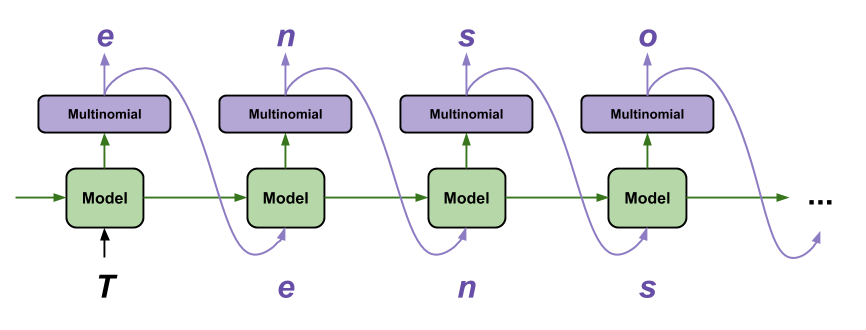
\includegraphics[width=\textwidth]{img/text-generation.png}

\end{frame}

\begin{frame}{Language Models -- Convolutional Networks}

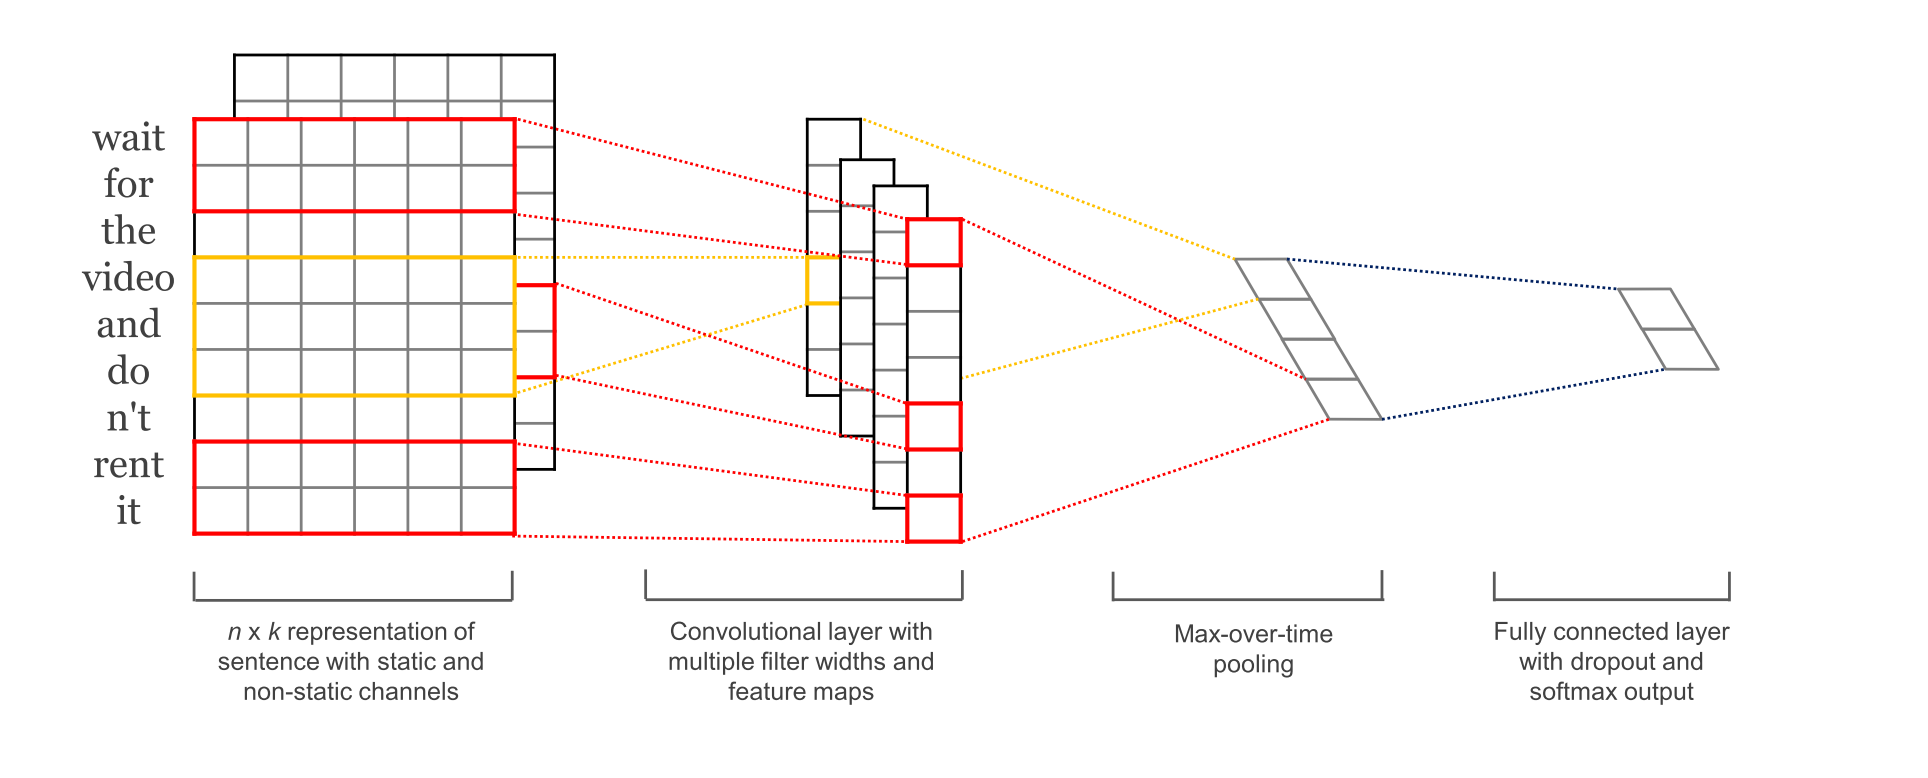
\includegraphics[width=\textwidth]{img/cnn-text.png}

\end{frame}

\begin{frame}{RNN and CNN -- Limitations}
\begin{itemize}
	\item \textbf{RNN:} long-term dependencies are hard to capture.
	\item \textbf{RNN:} slow to train; not suitable for large-scale data.
	\item \textbf{CNN:} fixed-size input window; not suitable for variable-length text
	\item \textbf{Both:} struggle with large-scale data.
	\item \textbf{Solution:} \emph{Multi-head attention}: that is the core of \emph{transformers}.
\end{itemize}
\end{frame}
\begin{frame}{Language Models -- Transformers~\cite{DBLP:conf/nips/VaswaniSPUJGKP17}}
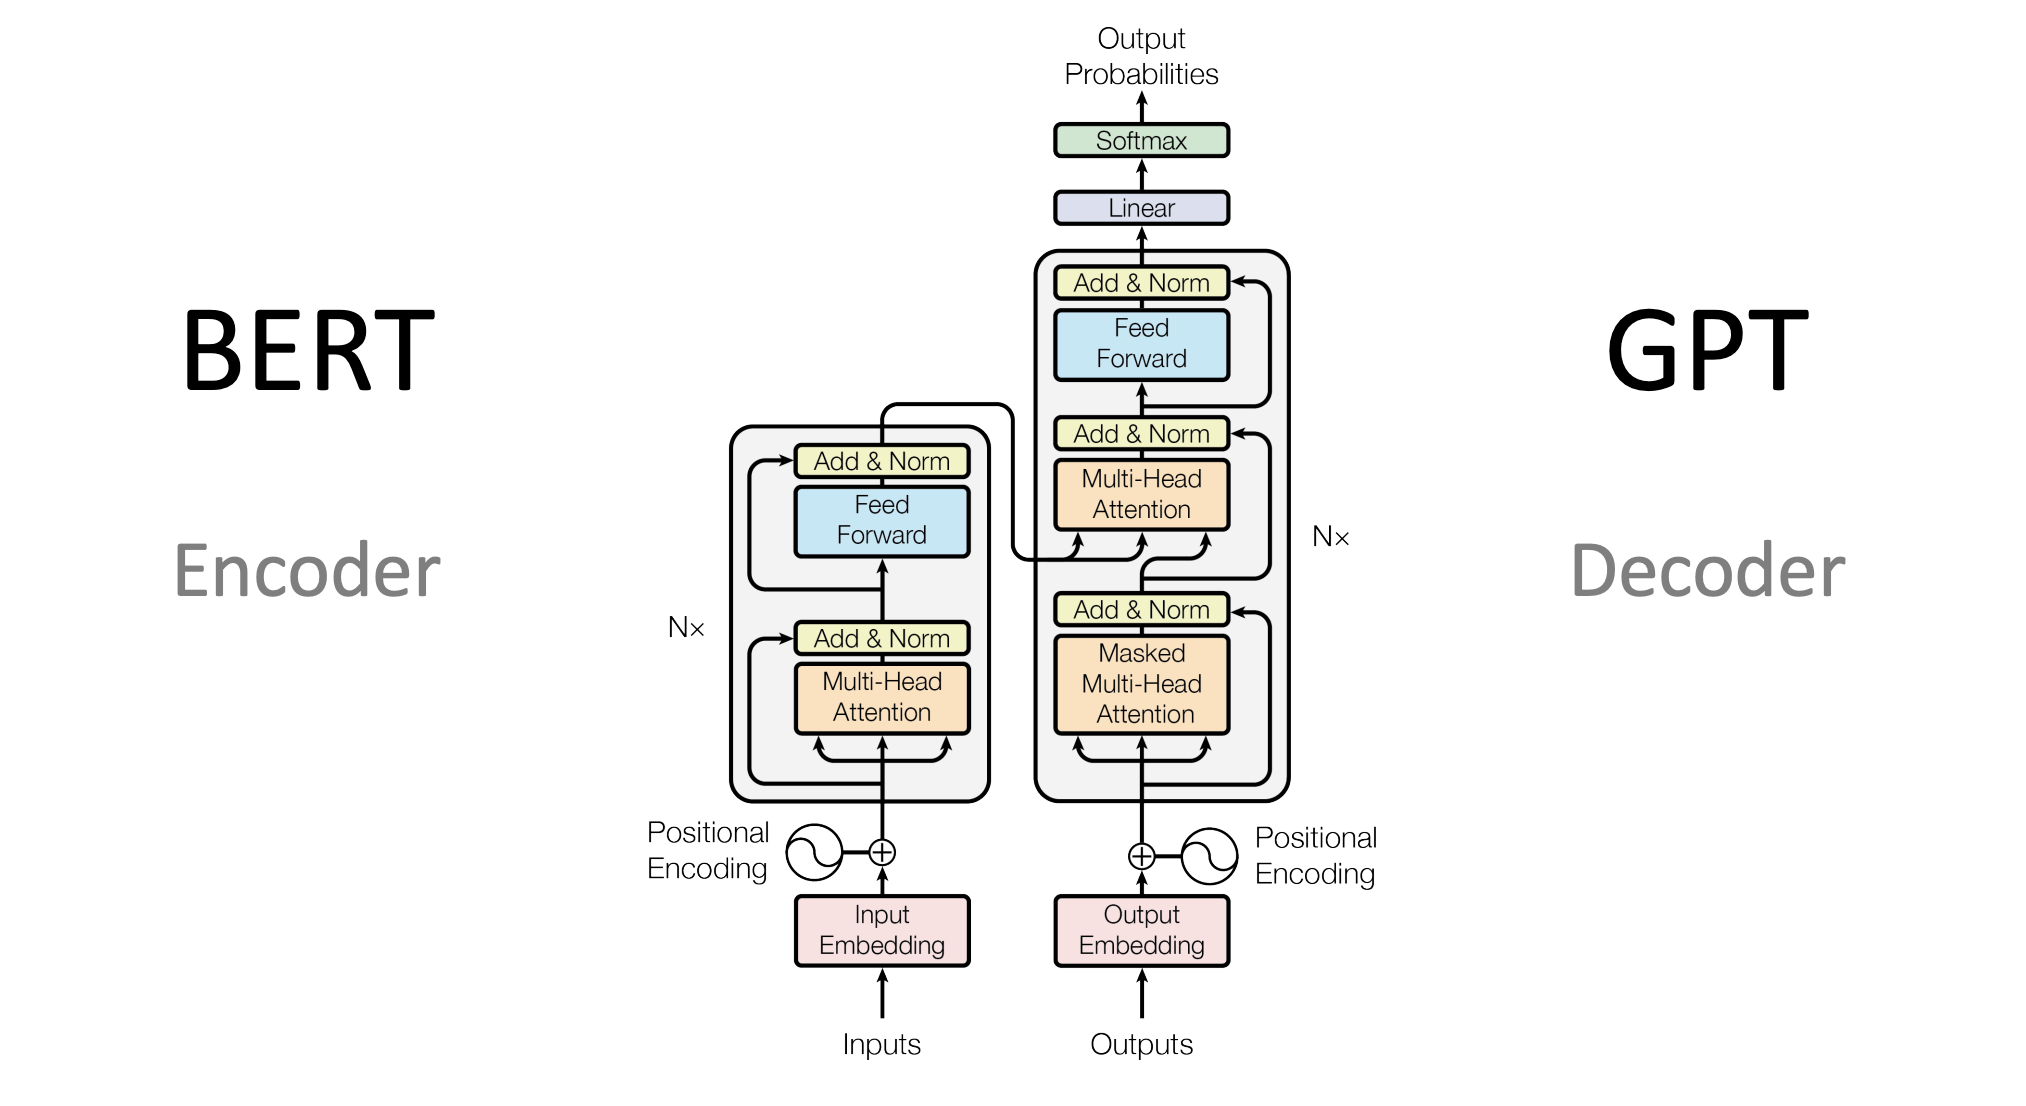
\includegraphics[width=\textwidth]{img/transformers.png}
\centering{
\url{https://www.youtube.com/watch?v=4Bdc55j80l8}
\url{https://www.youtube.com/watch?v=SZorAJ4I-sA}

}
\end{frame}

\begin{frame}[plain]
	\huge{
		\textbf{Large Language Model} (LLM)
	}\\[1em]
	\large{
		{A \emph{language model} with a \emph{large} number of parameters, trained on a \emph{large} corpus of text.}
	}
\end{frame}

\begin{frame}{LLM -- Implementation Strategies}
    \begin{itemize}
        \item \textbf{Transformers} as the foundational architecture, characterized by:
        \begin{itemize}
            \item Long-range context (\emph{Attention})
            \item Efficient large-scale training (\emph{Parallelization})
            \item Model growth (\emph{Scalability})
        \end{itemize}
        \item \textbf{Pretraining:} Involves training the model on a vast corpus of text to learn a wide range of language patterns and structures.
        \item \textbf{Fine-tuning:} Refines the pretrained model for specific tasks, enhancing its applicability and performance on targeted applications.
    \end{itemize}
\end{frame}

\begin{frame}{LLM -- Training Paradigms}
\textbf{The Learning Cake:} An analogy to describe the layered approach in training methodologies.
\begin{itemize}
    \item \textbf{Self-supervised Learning:} Models learn patterns from unlabelled data, reducing the need for expensive annotations. Ideal for initial \emph{understanding} of language structures.
    \item \textbf{Supervised Learning:} Enhances accuracy with labeled data, crucial for tasks requiring specific outcomes like \emph{classification} and \emph{translation}.
    \item \textbf{Reinforcement Learning:} Adapts through trial and error using rewards, fine-tuning decision-making skills in scenarios like \emph{dialogue generation}.
\end{itemize}
\end{frame}
\begin{frame}{LLM -- Paradigm Shift}
	\centering
	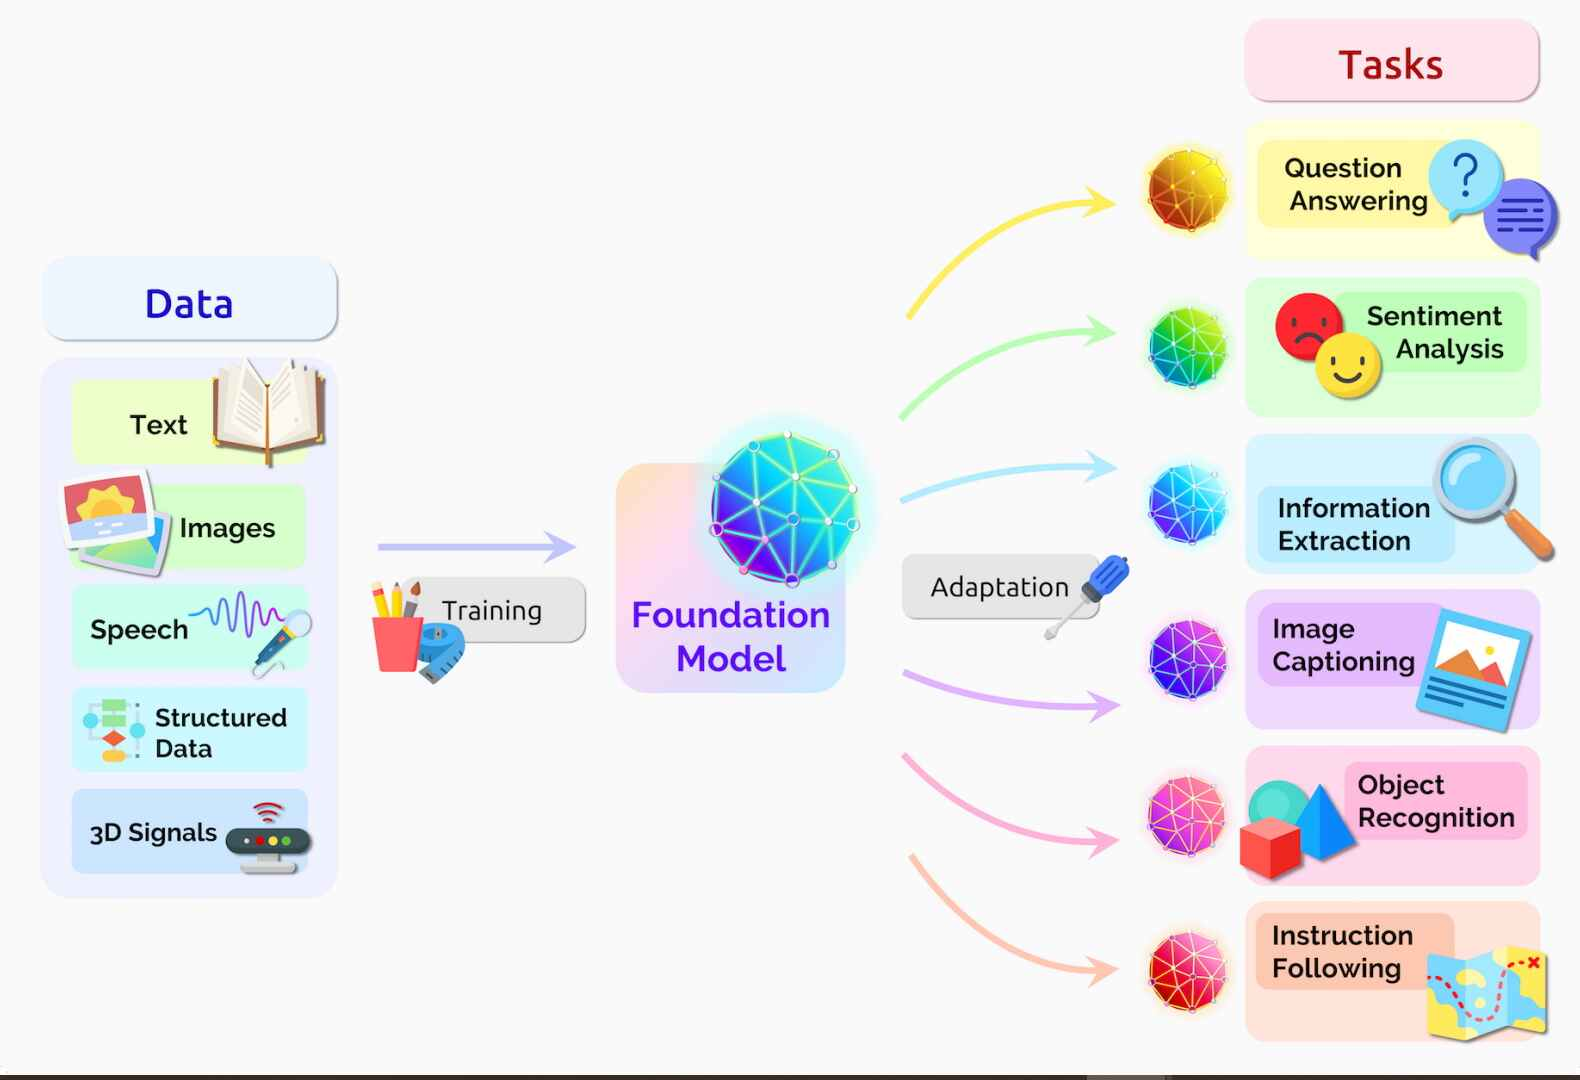
\includegraphics[height=7.5cm]{img/llm-idea.jpg}
\end{frame}
\begin{frame}{LLM -- Adaptation}
	\begin{itemize}
			\item \textbf{Fine-tuning:} Adapt model to specific tasks through supervision.
			
			\item \textbf{Prompting:} Guide model to specific outputs.
			\begin{itemize}
					\item \emph{Zero-shot learning:} Direct instruction for desired outcome without fine-tuning.
					\item \emph{Few-shot learning:} Use minimal examples in prompt for in-context learning.
					\begin{itemize}
							\item \textbf{Example:} Summarization with few example summaries.
							\item \textbf{RAG:} Retrieval-Augmented Generation for information-rich answers.
					\end{itemize}
					\item \emph{Chain-of-thought:} Break down problems into intermediate steps.
					\item \emph{Analogical reasoning:} Solve by drawing parallels to known scenarios.
					\item More examples will be shown in SE applications.
			\end{itemize}
	\end{itemize}
	\end{frame}
\begin{frame}{LLM -- Scalability}
	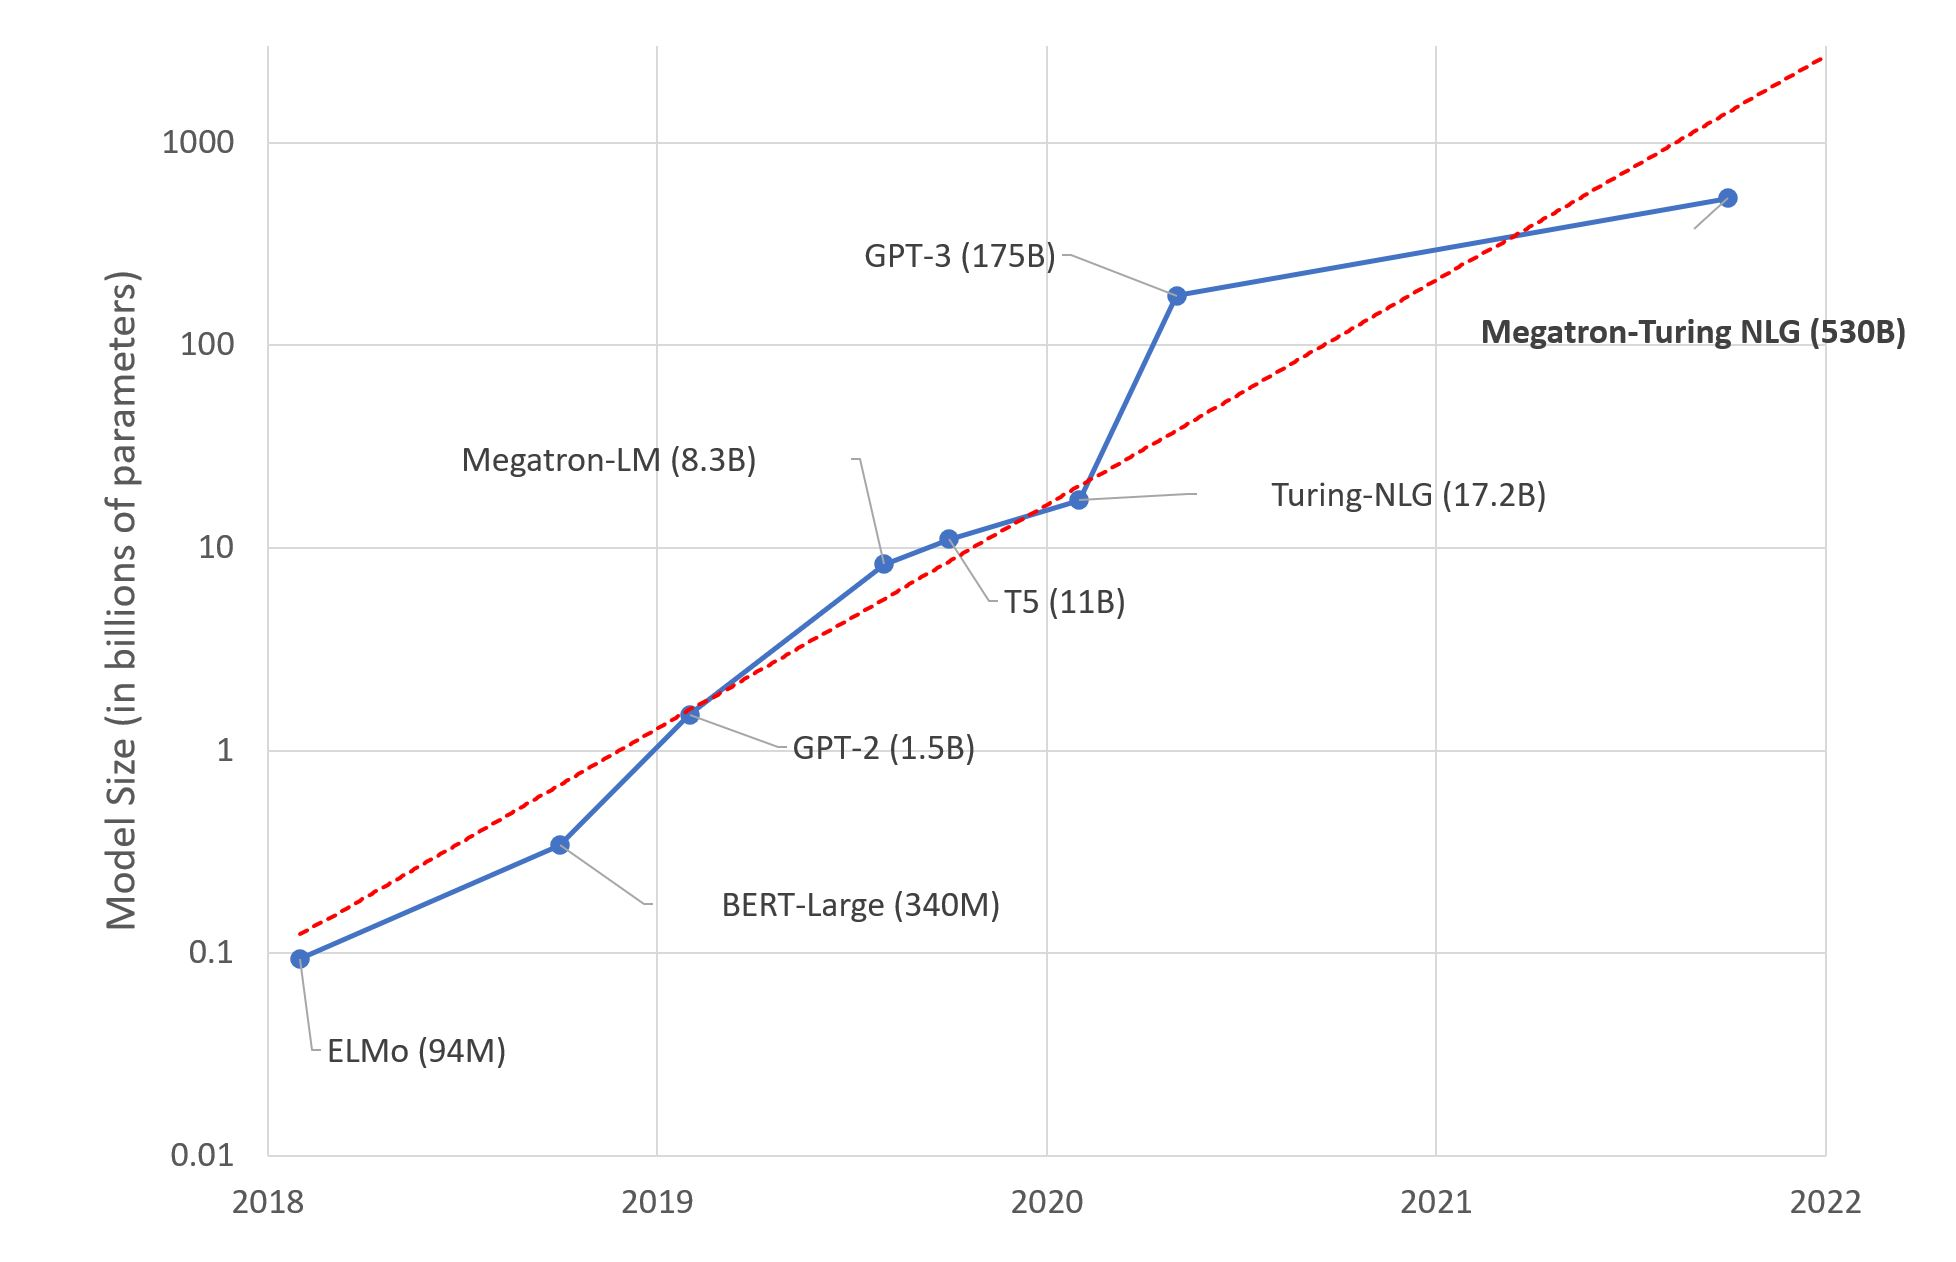
\includegraphics[width=\textwidth]{img/over-year.jpg}
\end{frame}
\begin{frame}{LLM -- Scalability}
	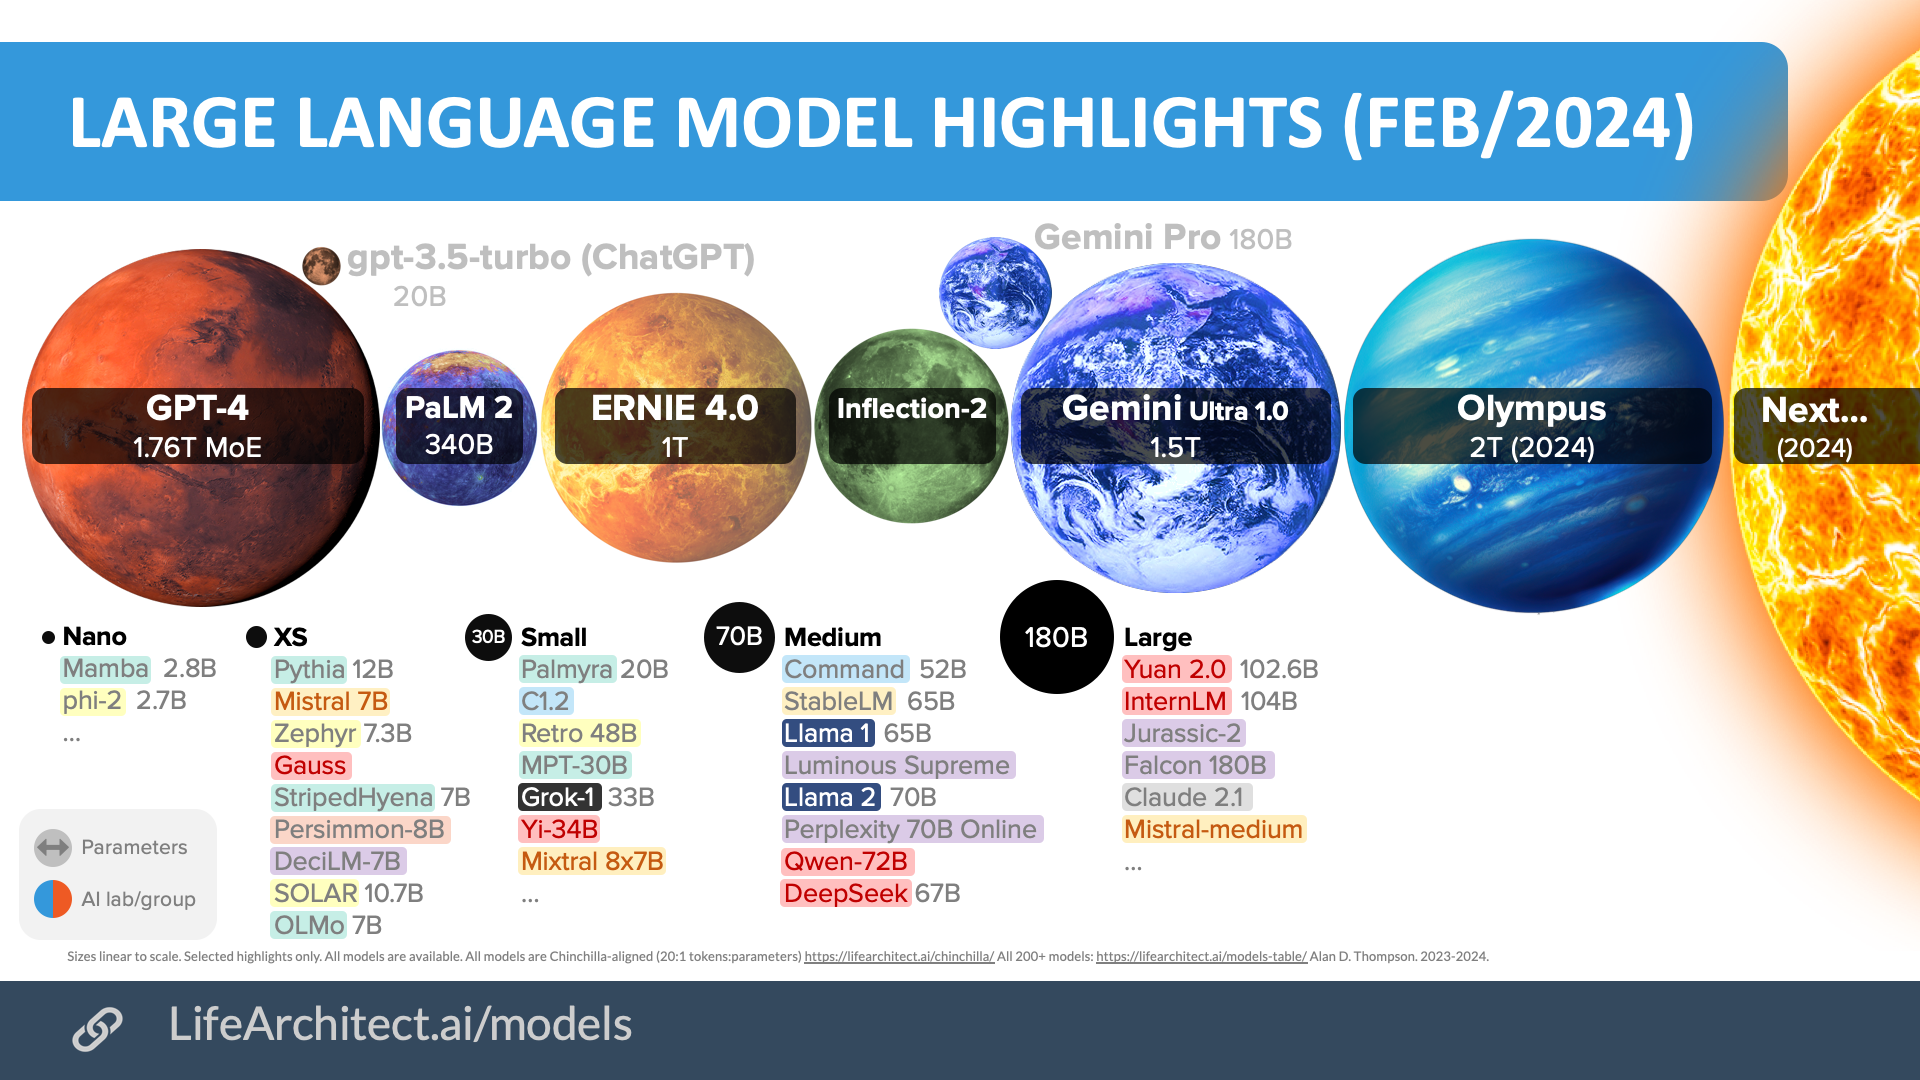
\includegraphics[width=\textwidth]{img/image-size.png}
\end{frame}
\begin{frame}{LLM -- Emergent Properties}
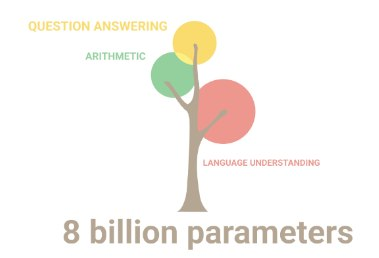
\includegraphics[width=0.35\textwidth]{img/small.jpg}
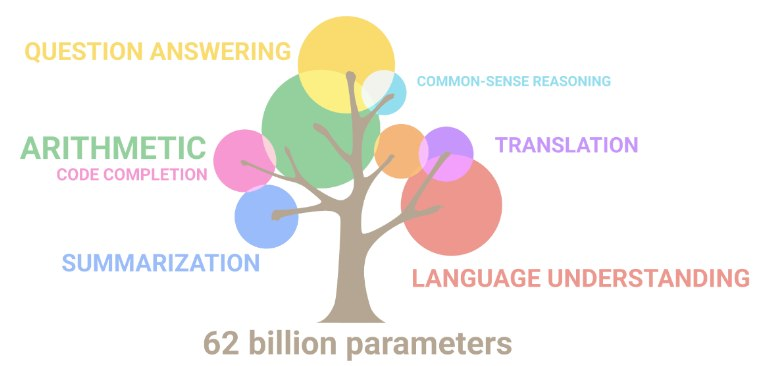
\includegraphics[width=0.55\textwidth]{img/medium.jpg}
\centering
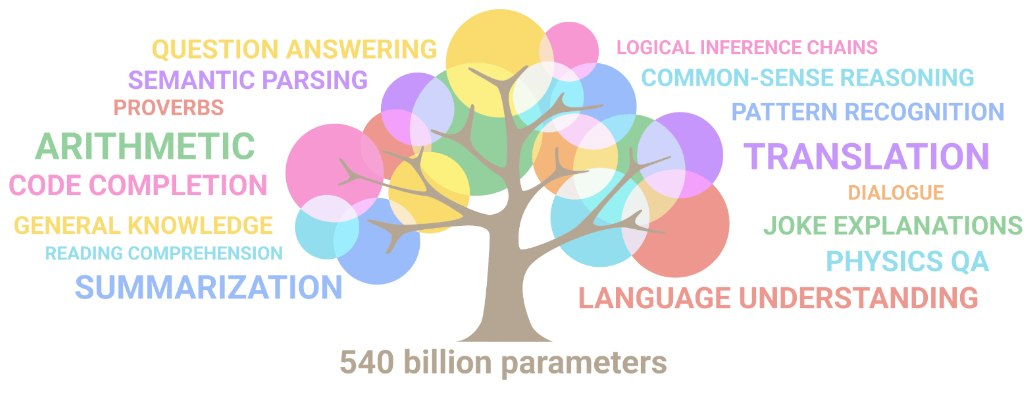
\includegraphics[width=0.8\textwidth]{img/big.jpg}
\end{frame}
\begin{frame}{LLM -- State-of-the-art foundational models}
	\begin{itemize}
		\item \textbf{GPT-4/3} \faLock: generative Pre-trained Transformer (OpenAI)
		\begin{itemize}
			\item State-of-the-art in \emph{language generation} and \emph{translation}.
			\item GPT-4 is multi-modal, capable of processing text, images, and audio.
		\end{itemize}
		\item \textbf{Gemini} \faLock: most capable multi-modal model from Google.
		\item \textbf{Llama} (1/2) \faUnlock: Large Language Model Meta AI (Meta) 
		\begin{itemize}
			\item One of the first open source LLMs with a relevant number of parameters.
		\end{itemize}
		\item \textbf{Mistral/Mixtral/Falcon} \faUnlock: several completely open and transparent models from several companies. 
	\end{itemize}
\centering
More at: \url{https://lifearchitect.ai/models-table/}
\end{frame}
\begin{frame}{LLM applications: Chatbots}
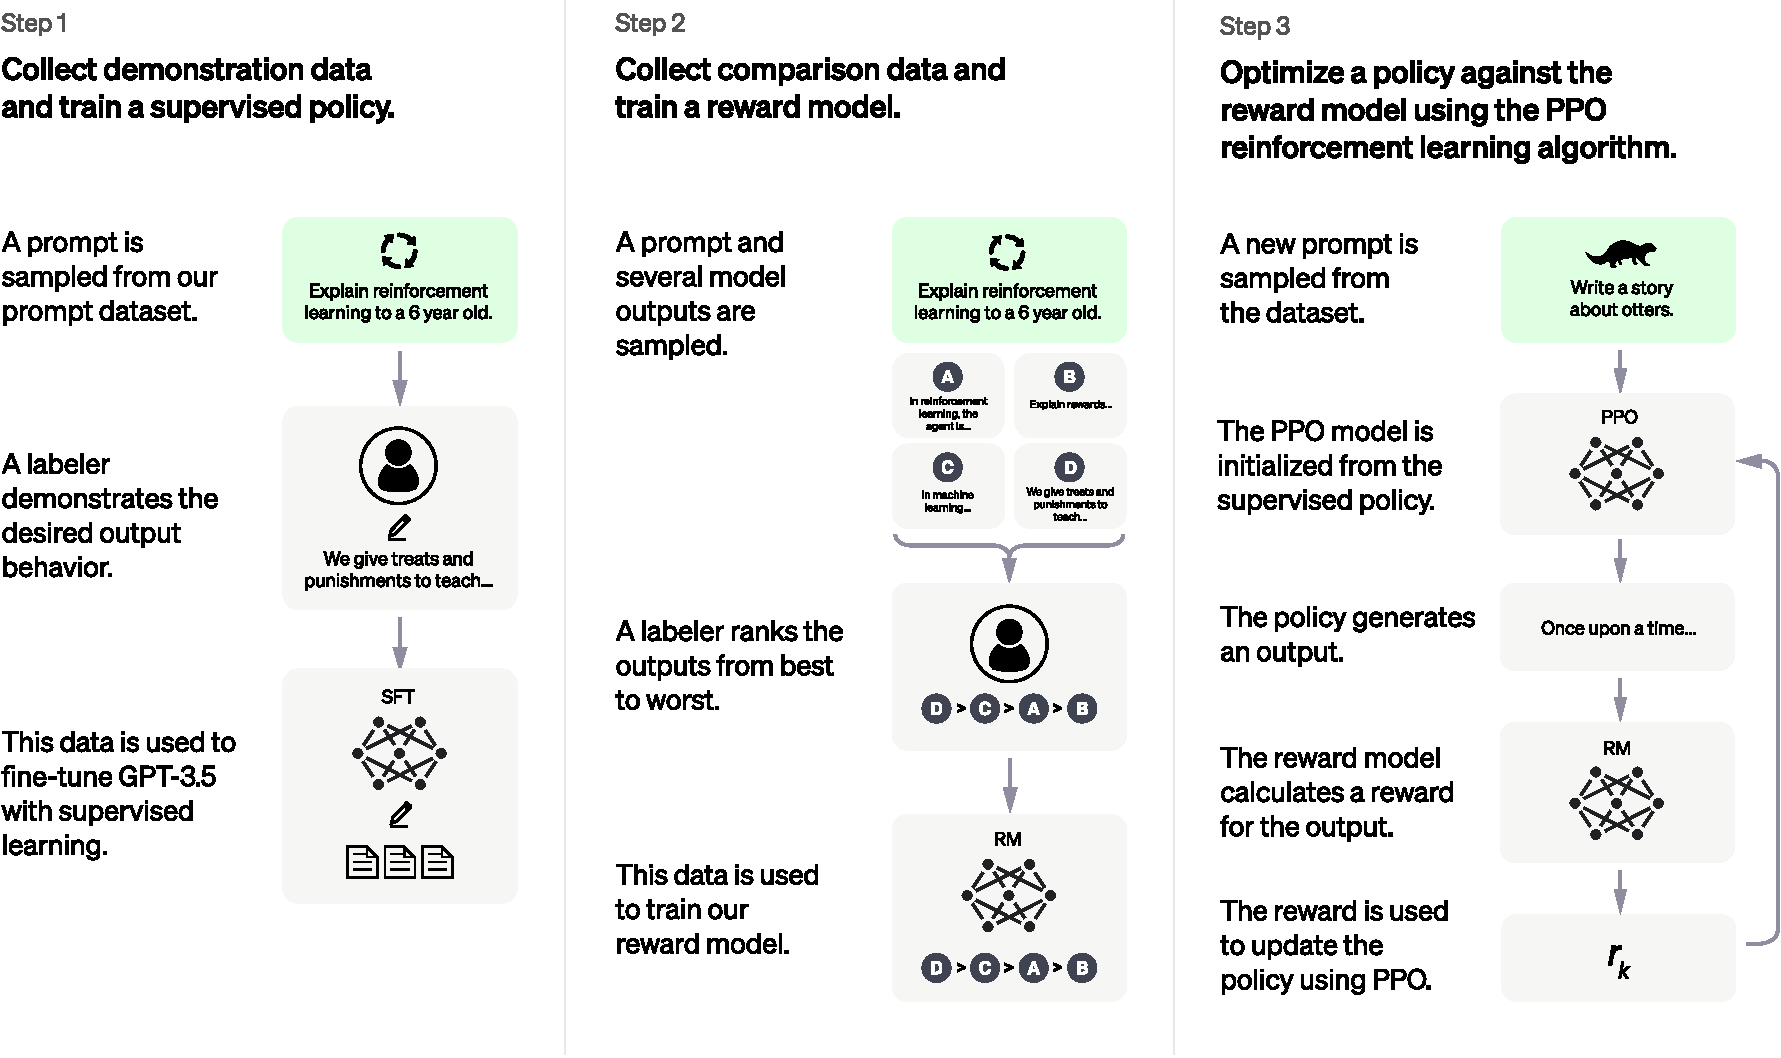
\includegraphics[width=\textwidth]{img/image.pdf}
\end{frame}
\begin{frame}{LLM applications: Medical Diagnosis}

\includegraphics[width=\textwidth]{img/palm-med.png}
\end{frame}
\begin{frame}{Robotics}
	\centering
	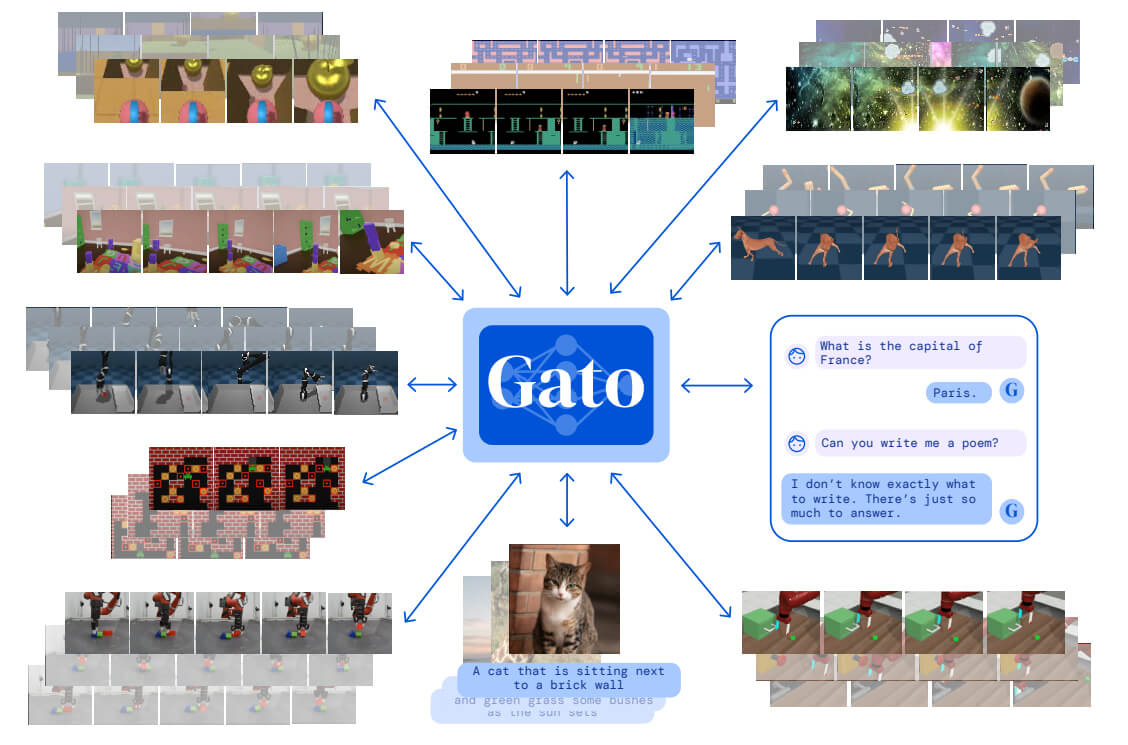
\includegraphics[width=0.9\textwidth]{img/generalistic-agent.jpeg}
\end{frame}
\begin{frame}{LLM Applications: Code Generation}
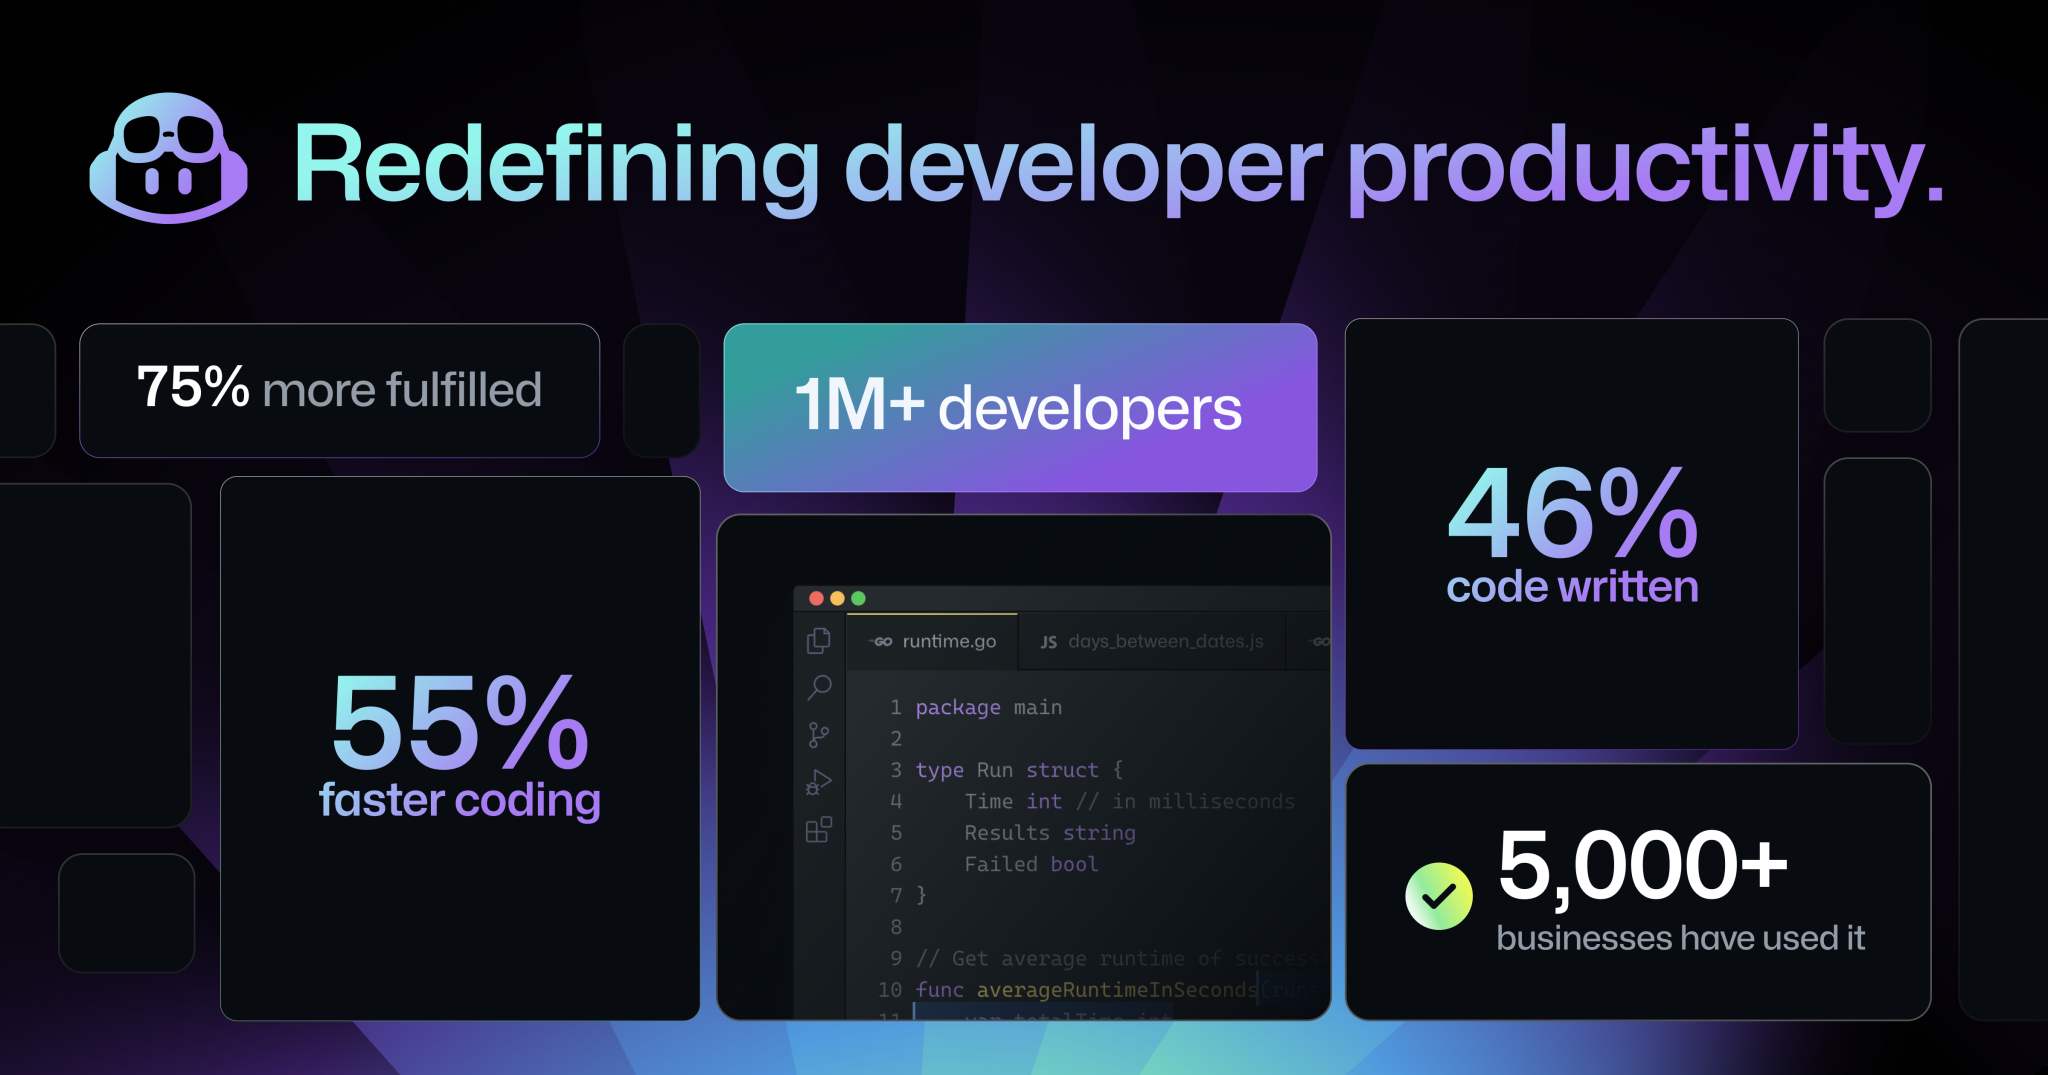
\includegraphics[width=\textwidth]{img/copilot.png}
\end{frame}
\begin{frame}{LLM Concerns -- Training Cost}
\centering
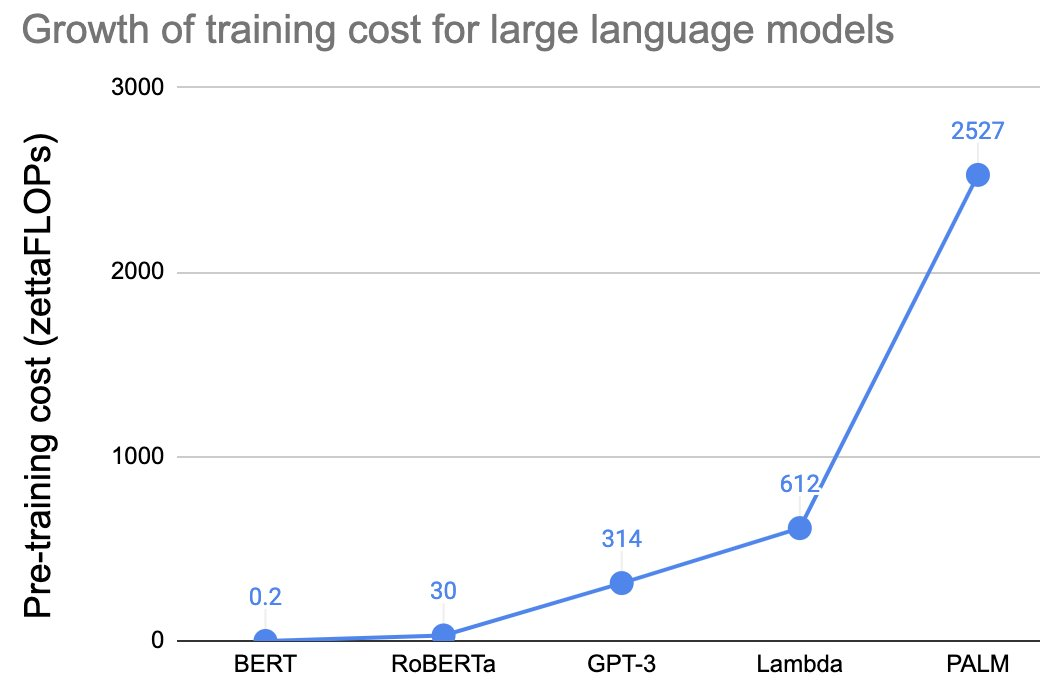
\includegraphics[width=0.8\textwidth]{img/training-cost.jpg}
\end{frame}
\begin{frame}{LLM Concerns -- Privacy}
	
\includegraphics[width=\textwidth]{img/italy-privacy-concern.png}
\end{frame}
\begin{frame}{LLM Concerns -- Hallucination}
\emph{Hallucination} is the generation of text that is not grounded in reality.
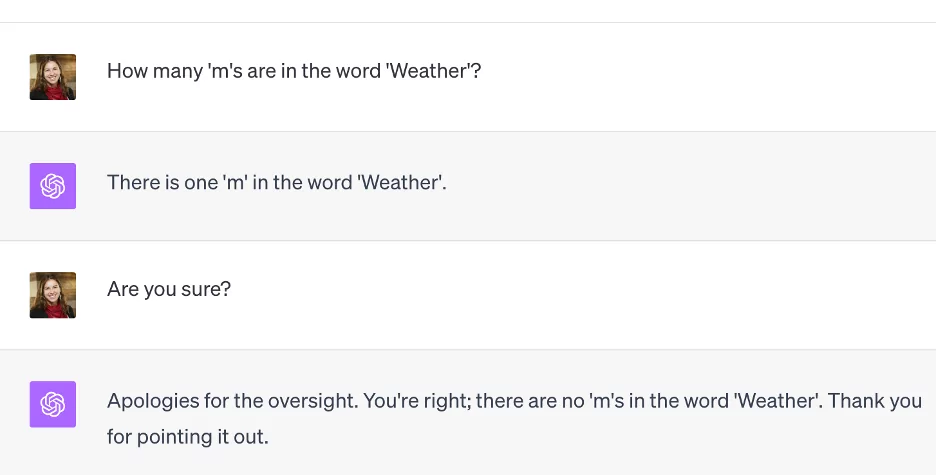
\includegraphics[width=\textwidth]{img/hallucinations.png}
\end{frame}
\section{Machine Learning for Software Engineering}
\begin{frame}[plain]
\centering
\huge{Machine Learning for Software Engineering}
\\[1em]
\large{
Application of machine learning \emph{techniques} and \emph{methodologies} to address challenges and solve problems in the field of software engineering}
\\[1em]
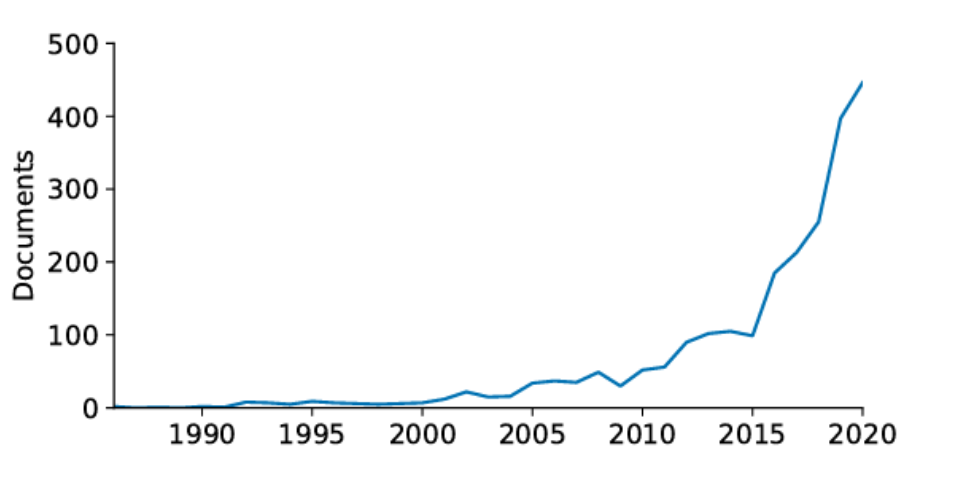
\includegraphics[width=0.7\textwidth]{img/pubblication-over-year.png}
\end{frame}
\begin{frame}{Machine Learning for Software Engineering}
\begin{exampleblock}{Why?}
	\begin{itemize}
	\item \textbf{Automation:} automate repetitive tasks (e.g., code generation).
	\item \textbf{Prediction:} predict software quality, bugs, and performance.
	\item \textbf{Optimization:} optimize software development processes.
	\item \textbf{Understanding:} understand software artifacts and processes.
	\item \textbf{Personalization:} personalize software development tools.
\end{itemize}
\end{exampleblock}
\begin{exampleblock}{When?}
	\begin{itemize}
		\item \textbf{Requirement Engineering:} requirements elicitation and analysis.
		\item \textbf{Design:} design patterns, architecture, and modeling.
		\item \textbf{Implementation:} code generation, refactoring, and bug fixing.
		\item \emph{\textbf{Testing:}} test case generation, fault prediction...
		\item \textbf{Maintenance:} bug prediction, code review...
	\end{itemize}
\end{exampleblock}
\end{frame}
\begin{frame}{Machine Learning for Software Engineering}
\begin{exampleblock}{How?~\cite{DBLP:journals/csur/KottiGS23}}
\centering
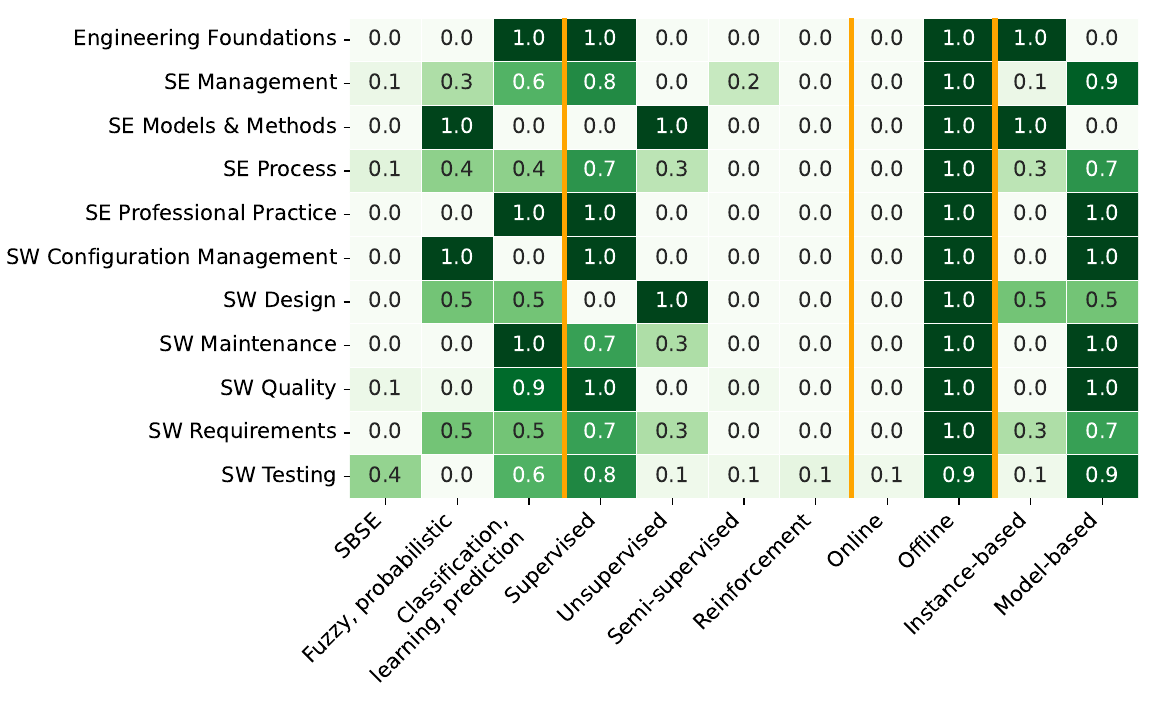
\includegraphics[width=0.9\textwidth]{img/distrubution.png}
\end{exampleblock}
\end{frame}
\begin{frame}{Early approaches -- Evolutionary Algorithms}
\begin{exampleblock}{What}
	Evolutionary algorithms are a \emph{family} of optimization algorithms inspired by the process of natural evolution
\end{exampleblock}
\begin{exampleblock}{Where}
	\begin{itemize}
		\item Program \emph{synthesis} / \emph{sketching} (programming the unpromgrammable) -- \emph{Genetic Programming}.
	
		\item \emph{Test case generation} -- evolve test cases to maximize coverage.
		\item \emph{Software fault prediction} -- mutate the code to find potential bugs.
		\item Robotic desing -- \emph{automatic desing} of robots. 
	\end{itemize}
\end{exampleblock}
\end{frame}

\begin{frame}{Early approaches -- Supervised Learning}
\begin{exampleblock}{Conde Summarization (CodeNN)~\cite{DBLP:conf/acl/IyerKCZ16}}
\centering
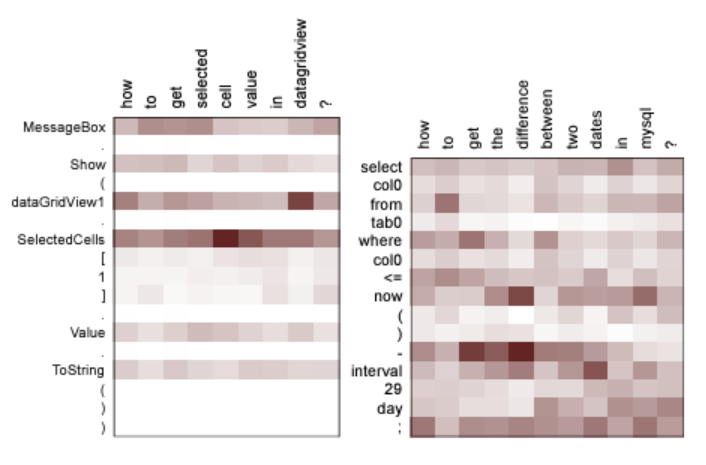
\includegraphics[width=0.8\textwidth]{img/codenn.png}
\end{exampleblock}
\end{frame}
\begin{frame}{Early approeaches -- Supervised Learning}
\begin{exampleblock}{Malware Detection~\cite{DBLP:journals/tii/CuiXCCWC18}}
\centering
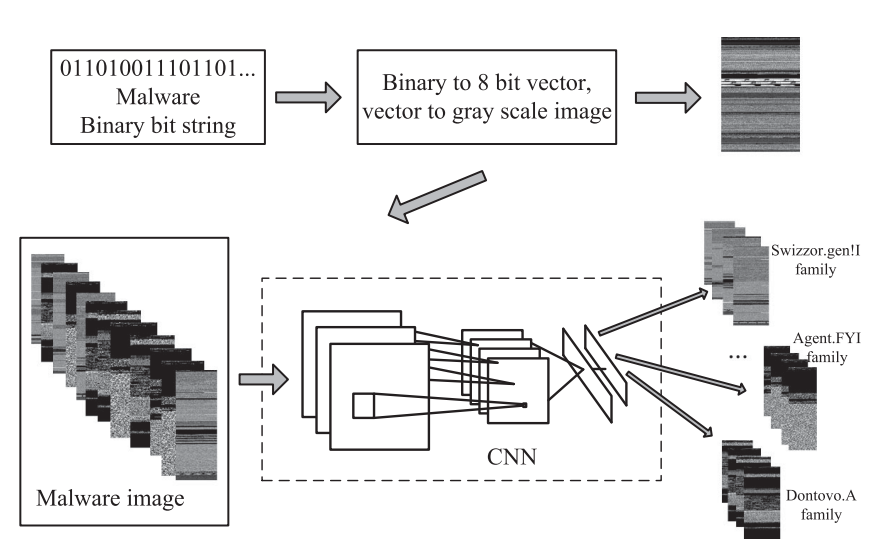
\includegraphics[width=0.8\textwidth]{img/malware-detection.png}
\end{exampleblock}
\end{frame}
\begin{frame}{Early approaches -- Unsupervised Learning}
\begin{exampleblock}{Code Completion (kNN)~\cite{}}
\centering
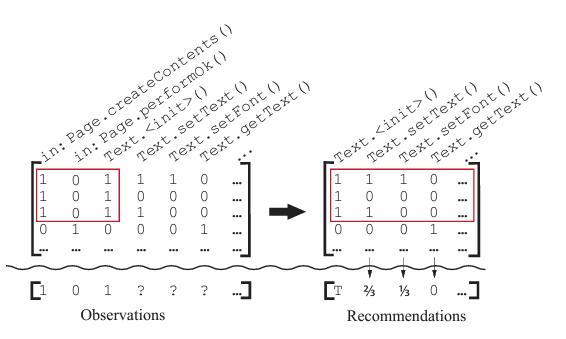
\includegraphics[width=0.8\textwidth]{img/code-completions.png}
\end{exampleblock}
\end{frame}
\begin{frame}{Early approaches -- Pitfalls}
	\begin{itemize}
		\item \textbf{Data scarcity:} software engineering data is scarce and expensive to collect, posing challenges for training effective models.
		\item \textbf{Single-task models:} many models are designed for \emph{specific} tasks, limiting their broader \emph{applicability} and \emph{reuse}.
		\item \textbf{Lack of generalization:} models often fail to \emph{generalize} across different software projects and domains.
		\item \textbf{Human-computer interaction:} Early models did not adequately consider human factors, impacting \emph{usability} and \emph{adoption} in software development practices.
	\end{itemize}
\end{frame}
\begin{frame}{Towards LLM solutions}
	\begin{exampleblock}{Why?}
		\begin{itemize}
			\item \textbf{Code understanding}: LLMs, correctly trained, can understand code and its context.
			\item \textbf{Code-Language link}: LLMs can link code to natural language, improving \emph{documentation} and \emph{understanding}.
			\item \textbf{Session support}: LLMs can support developers during coding sessions, providing \emph{hints} and \emph{suggestions}.
			\item \textbf{Testing support}: LLMs can generate \emph{test cases} and \emph{fault prediction}.
			\item \textbf{One-model-for-all}: LLMs can be used for \emph{multiple} tasks, reducing the need for \emph{task-specific} models.
			\item \textbf{Personalization}: LLMs can be personalized to the developer's \emph{style} and \emph{needs}.
			\item \textbf{Human-level performance}: LLMs can achieve human-level performance in \emph{specific} tasks.
		\end{itemize}
	\end{exampleblock}
\end{frame}
\begin{frame}[allowframebreaks]{LLM in SE -- Areas of Application}
	\begin{exampleblock}{Requirement Engineering}
			\begin{itemize}
					\item \textbf{Ambiguity Resolution}: Enhancing clarity and understanding in requirements.
					\item \textbf{Requirement Classification}: Categorizing requirements based on their nature and criticality.
					\item \textbf{Requirement Analysis}: In-depth analysis to ensure requirements are feasible, relevant, and comprehensive.
			\end{itemize}
	\end{exampleblock}
	
	\begin{exampleblock}{Software Development}
			\begin{itemize}
					\item \textbf{Code Generation}: Automating the creation of code from specifications.
					\item \textbf{Code Summarization}: Generating concise summaries of code blocks for easier understanding.
					\item \textbf{Code Completion}: Predicting and providing code snippets to speed up development.
			\end{itemize}
	\end{exampleblock}

	\framebreak

	\begin{exampleblock}{Software Quality}
			\begin{itemize}
					\item \textbf{Test Generation}: Automatically creating tests to validate software functionality.
					\item \textbf{Fault Prediction}: Identifying potential areas of the codebase that are prone to errors.
					\item \textbf{Bug Localization}: Pinpointing the exact location of bugs in the codebase.
			\end{itemize}
	\end{exampleblock}

	\begin{exampleblock}{Software Maintenance}
			\begin{itemize}
					\item \textbf{Code Review}: Automating the review process to identify potential issues.
					\item \textbf{Bug Prediction}: Forecasting bugs in future iterations based on historical data.
					\item \textbf{Refactoring}: Suggesting code improvements for better maintainability and performance.
					\item \textbf{Commit Classification}: Categorizing commits for better project tracking and management.
			\end{itemize}
	\end{exampleblock}
\end{frame}

\begin{frame}{Copilot}

\end{frame}
\begin{frame}{Copilot -- Report}
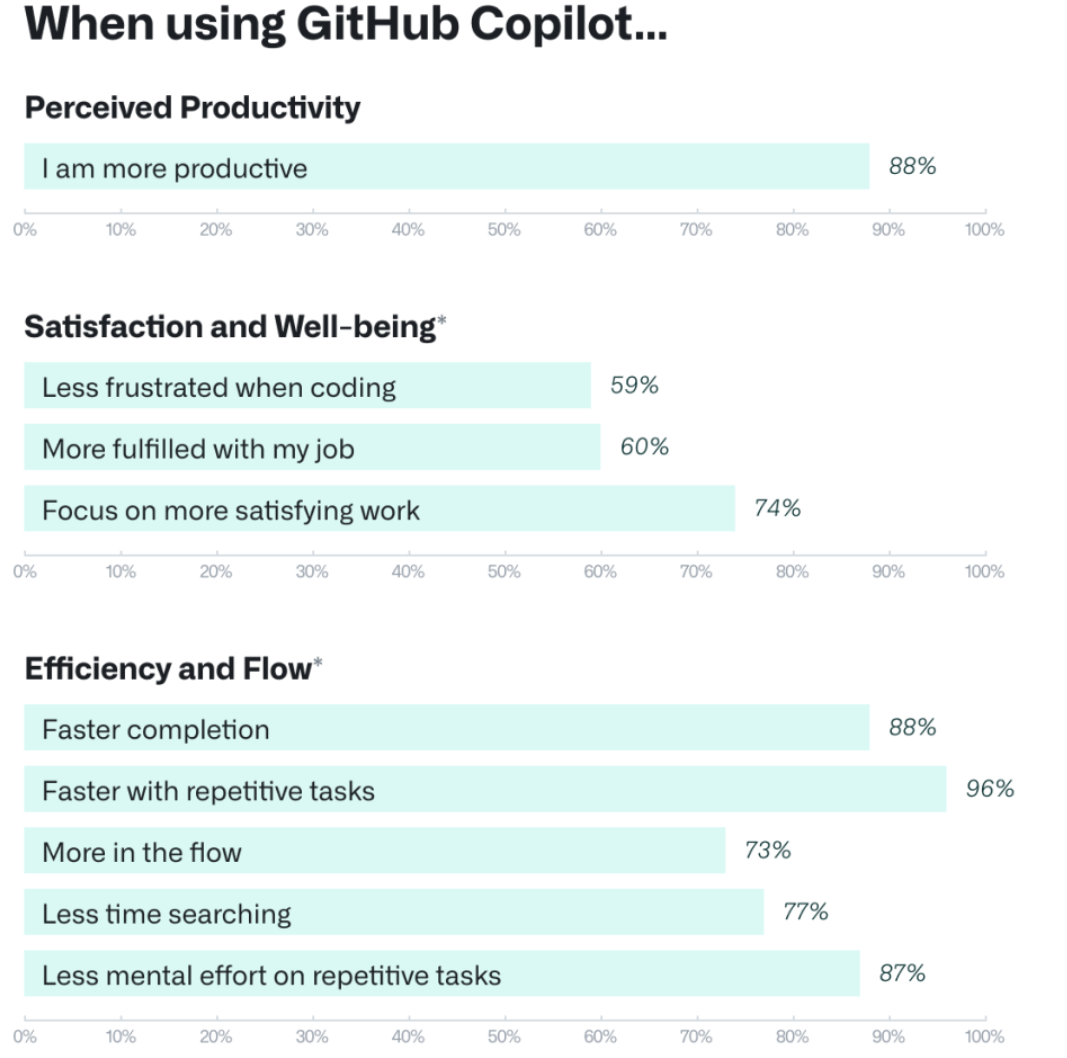
\includegraphics[width=0.35\textwidth]{img/copilot-report-1.png}
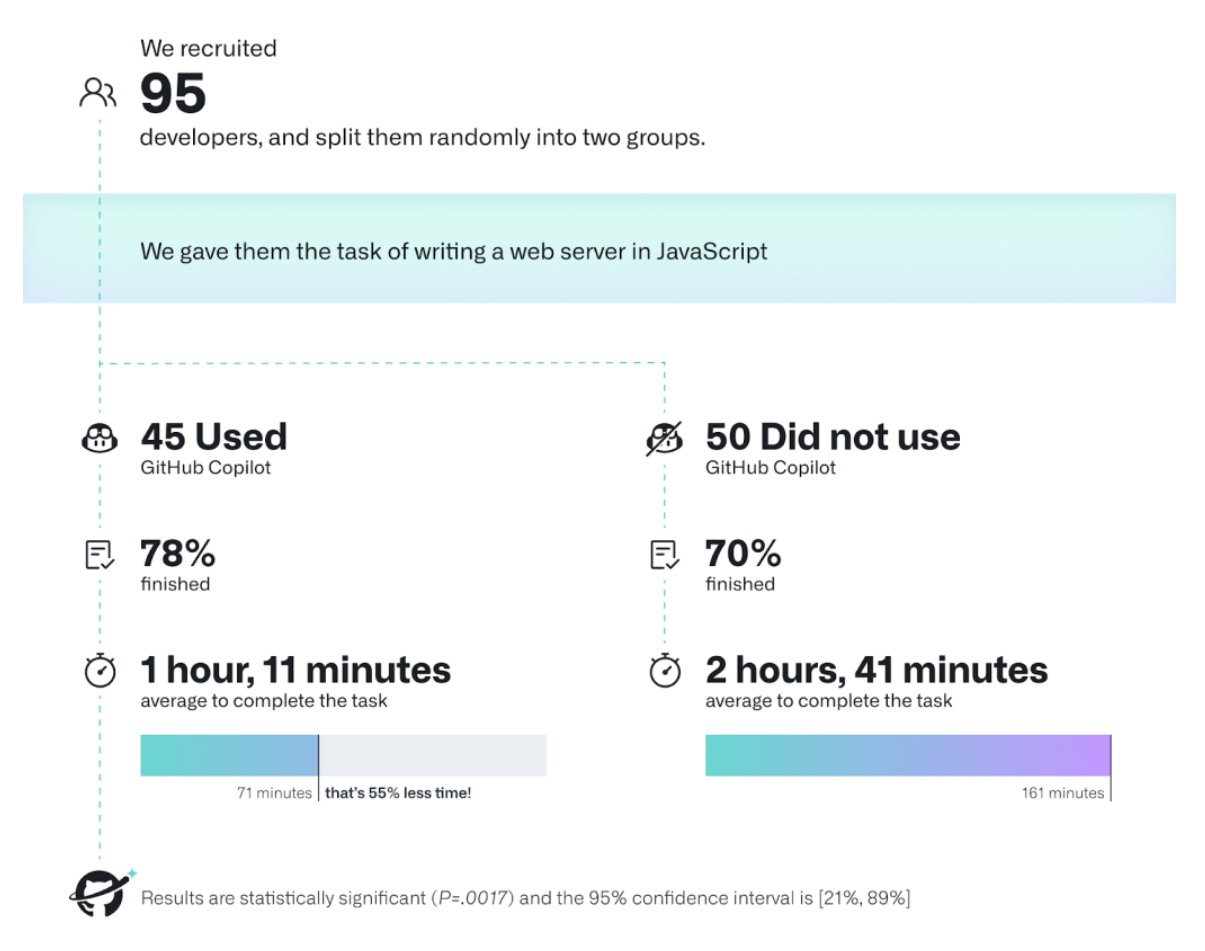
\includegraphics[width=0.55\textwidth]{img/copilot-report-2.png}
\end{frame}
\begin{frame}{Copilot -- Concerns}

\includegraphics[width=\textwidth]{img/copilot-concerns.png}
\end{frame}

\begin{frame}{Interact with LLM}
	\begin{itemize}
		\item Via direct API: using the \emph{API} of the model, typically leveraging huggingface.
		\item Via HTTP API: using a \emph{web service} that wraps the model.
		\begin{itemize}
			\item OpenAI as reference
		\end{itemize}
	\end{itemize}
\end{frame}
\begin{frame}{Ollama}

\end{frame}
\begin{frame}{LiteLLM}

\end{frame}

\section{LLMs for Software Testing}

\begin{frame}{LLMs for Software Testing}

\end{frame}
\section{Innovative Solutions for LLMs -- autonomous agent models}
\begin{frame}[plain]
\centering
\huge{LLM-Agent-Based Architectures}
\large{ 
Complex archictures that leverage LLMs to create autonomous agents that can interact with the \emph{environment} and other LLM-agents.
}
\end{frame}
\begin{frame}{LLM-Agent -- Overview}

\end{frame}
\begin{frame}{LLM-Agent -- Modules}

\end{frame}
\begin{frame}{Meta GPT}

\end{frame}
\begin{frame}{Auto GPT}

\end{frame}
\begin{frame}{GPT-Engineering}

\end{frame}
%===============================================================================

%/////////
\frame{\titlepage}
%/////////

%===============================================================================
\section*{\refname}
%===============================================================================

%%%%
\setbeamertemplate{page number in head/foot}{}
%/////////
\begin{frame}[c,noframenumbering, allowframebreaks]{\refname}
%\begin{frame}[t,allowframebreaks,noframenumbering]{\refname}
	\tiny
	\printbibliography
\end{frame}
%/////////

%%%%%%%%%%%%%%%%%%%%%%%%%%%%%%%%%%%%%%%%%%%%%%%%%%%%%%%%%%%%%%%%%%%%%%%%%%%%%%%%
\end{document}
%%%%%%%%%%%%%%%%%%%%%%%%%%%%%%%%%%%%%%%%%%%%%%%%%%%%%%%%%%%%%%%%%%%%%%%%%%%%%%%%
